% =====================================================================
%  Proposal PERURI Chip Hackathon 2026
%  Secure Battery Identity Chip
%  Kompilasi: pdflatex main.tex (dua kali) atau latexmk -pdf main.tex
% =====================================================================
\documentclass[11pt,a4paper]{article}

% ---------- Tata letak & huruf (meniru template Google Docs) ----------
\usepackage[a4paper,margin=2.5cm]{geometry}
\usepackage[T1]{fontenc}
\usepackage[utf8]{inputenc}
\usepackage[scaled=0.95]{helvet}
\renewcommand{\familydefault}{\sfdefault}
\usepackage{microtype}
\usepackage{amsmath}
\setlength{\parindent}{0pt}
\setlength{\parskip}{6pt}
\linespread{1.08}

\usepackage[table]{xcolor}
\usepackage{graphicx}
\usepackage{tabularx}
\usepackage{array}
\usepackage{enumitem}
\usepackage{titlesec}
\usepackage{caption}
\usepackage{float}
\usepackage{tcolorbox}
\usepackage{pifont}
\newcommand{\cmark}{\textcolor{okline}{\ding{51}}}
\newcommand{\xmark}{\textcolor{badline}{\ding{55}}}
\newcommand{\pmark}{\textcolor{subtle}{\ding{108}}}
\usepackage{fancyhdr}
\usepackage{tikz}
\usetikzlibrary{positioning,arrows.meta,fit,backgrounds,calc}
\usepackage[hidelinks]{hyperref}

% ---------- Warna ----------
\definecolor{hdrgreen}{HTML}{E6EFC5}   % header tabel seperti template
\definecolor{subtle}{HTML}{6B7280}
\definecolor{todo}{HTML}{DC2626}
\definecolor{secfill}{HTML}{EEF2FF}
\definecolor{secline}{HTML}{4338CA}
\definecolor{okfill}{HTML}{F0FDF4}
\definecolor{okline}{HTML}{16A34A}
\definecolor{badfill}{HTML}{FEF2F2}
\definecolor{badline}{HTML}{DC2626}

% ---------- Judul bagian ----------
\titleformat{\section}{\fontsize{19}{23}\selectfont\raggedright}{\thesection.}{0.4em}{}
\titleformat{\subsection}{\fontsize{15}{19}\selectfont\raggedright}{\thesubsection}{0.5em}{}
\titleformat{name=\section,numberless}{\fontsize{19}{23}\selectfont\raggedright}{}{0em}{}
\titlespacing*{\section}{0pt}{18pt}{6pt}
\titlespacing*{\subsection}{0pt}{14pt}{4pt}

\newcommand{\field}[1]{\textbf{#1}\par\nobreak}
\newcommand{\todo}[1]{\textcolor{todo}{\textbf{[#1]}}}
\newcommand{\hdr}[1]{\cellcolor{hdrgreen}\textbf{#1}}

\setlist[itemize]{leftmargin=1.4em,itemsep=2pt,topsep=2pt}
\setlist[enumerate]{leftmargin=1.6em,itemsep=2pt,topsep=2pt}
\captionsetup{font=small,labelfont=bf,labelsep=period}
\renewcommand{\figurename}{Gambar}
\renewcommand{\tablename}{Tabel}
\renewcommand{\refname}{}
\renewcommand{\arraystretch}{1.3}

\pagestyle{fancy}
\fancyhf{}
\renewcommand{\headrulewidth}{0pt}
\fancyfoot[C]{\footnotesize\color{subtle}Hackathon CHIP 2026 --- Secure Battery Identity Chip \quad|\quad \thepage}

% =====================================================================
\begin{document}

% =====================================================================
%  COVER (tidak dihitung dalam batas 6 halaman)
% =====================================================================
\begin{titlepage}
\thispagestyle{empty}
\vspace*{1.2cm}
{\large\color{subtle} PROPOSAL PESERTA HACKATHON CHIP 2026\par}
\vspace{2pt}
{\color{subtle} Kategori: IC Chip Design \& FPGA Implementation\par}
{\color{subtle} Topik 1: Secure Identity \& Security Element Chip\par}
\vspace{1.6cm}
{\fontsize{34}{40}\selectfont\bfseries Secure Battery\\[4pt] Identity Chip\par}
\vspace{10pt}
{\color{secline}\rule{3cm}{2.5pt}\par}
\vspace{10pt}
{\Large \emph{Secure Element} Berbasis PUF untuk Autentikasi Baterai\\ pada Ekosistem Tukar Baterai Kendaraan Listrik\par}

\vfill
\begin{tcolorbox}[colback=secfill!40, colframe=secline!60, boxrule=0.6pt, arc=3pt, left=10pt, right=10pt, top=8pt, bottom=8pt]
\small
\renewcommand{\arraystretch}{1.35}
\newcommand{\mail}[1]{{\footnotesize\color{subtle}#1}}
\begin{tabular*}{\linewidth}{@{\extracolsep{\fill}}>{\bfseries}l l r@{}}
Nama Tim & \todo{Nama Tim} & \\
Ketua & Guntur Sulistyo & \mail{guntursulistyo@mail.ugm.ac.id} \\
Anggota & Dimas Eryan Ahnaf Fahrezi & \mail{adimaseryanahnaffahrezi@mail.ugm.ac.id} \\
Anggota & Muhammad Muqtada Alhaddad & \mail{muhammadmuqtadaalhaddad@mail.ugm.ac.id} \\
Dosen Pembimbing & \multicolumn{2}{l}{Ir. Agus Bejo, S.T., M.Eng., D.Eng., IPM} \\
Institusi & Universitas Gadjah Mada & \\
\end{tabular*}
\end{tcolorbox}
\vspace{0.6cm}
{\color{subtle}Yogyakarta, Oktober 2026\par}
\end{titlepage}

\setcounter{page}{1}

% =====================================================================
\section{Executive Summary}

Setiap hari, pengendara motor listrik menukar baterai kosong dengan baterai penuh di stasiun penukaran hanya dalam hitungan menit. Baterai yang mereka bawa pulang bukan milik mereka: sebelumnya baterai itu mungkin telah dipakai banyak pengendara lain dan berpindah di antara beberapa operator. Saat menerima sebuah baterai, stasiun hanya bisa \emph{berasumsi} bahwa baterai tersebut asli dan catatan pemakaiannya benar, karena belum ada cara yang andal untuk membuktikannya. Celah ini berbahaya. Baterai palsu atau hasil rekondisi asal-asalan dapat lolos ke jaringan dan memicu kebakaran, sementara jumlah siklus pemakaian dapat diubah agar baterai tua tampak baru. \textbf{Model tukar baterai berdiri di atas kepercayaan, dan kepercayaan itu saat ini belum dapat diverifikasi.}

Kami mengusulkan \textbf{Secure Battery Identity Chip}, sebuah IP \emph{secure element} berukuran kecil yang ditanam di dalam pack baterai di samping \emph{Battery Management System} (BMS). Chip ini memberi setiap baterai identitas kriptografis yang berasal dari sifat fisik silikonnya sendiri: kunci diturunkan dari \emph{Ring-Oscillator Physical Unclonable Function} (RO-PUF) setiap kali chip menyala dan \textbf{tidak pernah disimpan} di memori. Stasiun memverifikasi keaslian melalui protokol \emph{challenge--response} HMAC-SHA-256 dengan \emph{nonce} sekali pakai, chip menandatangani log riwayat dari BMS, dan monitor \emph{glitch}/\emph{tamper} menghapus kunci begitu serangan fisik terdeteksi.

\begin{center}
\small
\renewcommand{\arraystretch}{1.35}
\begin{tabularx}{\linewidth}{|>{\raggedright\arraybackslash}p{3.3cm}|X|}
\hline
\hdr{Chip yang dirancang} & \emph{Secure element} tanpa memori non-volatil: RO-PUF + \emph{fuzzy extractor}, inti HMAC-SHA-256 (baseline TT07~\cite{tt07}), FSM autentikasi, dan monitor \emph{tamper} dengan respons \emph{zeroize}. \\ \hline
\hdr{Target pengguna} & Operator SPBKLU dan penyedia layanan sewa baterai; produsen baterai dan BMS; lembaga penjamin keaslian yang mengelola registri identitas perangkat. \\ \hline
\hdr{Dampak} & \textbf{Keselamatan:} baterai yang tidak dikenal ditolak sebelum diisi atau diserahkan. \textbf{Ekonomi:} riwayat baterai dapat dipercaya untuk penilaian nilai sisa, garansi, dan pemanfaatan ulang. \textbf{Kemandirian:} akar kepercayaan (\emph{root of trust}) dirancang di dalam negeri dan tidak bergantung pada satu vendor. \\ \hline
\hdr{Platform validasi} & DE10-Nano: \emph{fabric} Cyclone~V menjalankan chip; HPS (ARM) mengemulasikan BMS dan stasiun penukaran. \\ \hline
\hdr{Target terukur} & Autentikasi $<10\,\mu$s; area $<15\%$ ALM Cyclone~V tanpa DSP; kunci PUF stabil 100\% di seluruh kondisi uji; nol \emph{false accept} pada empat skenario serangan. \\ \hline
\end{tabularx}
\end{center}

Kebaruan usulan ini terletak pada perpaduan tiga sifat yang jarang hadir bersama pada chip autentikasi baterai: \textbf{kunci tanpa penyimpanan} (PUF), \textbf{respons terhadap serangan fisik di tingkat hardware}, dan \textbf{pemisahan peran verifikasi} ke registri pihak tepercaya sehingga stasiun tidak pernah memegang kunci baterai mana pun. Hasilnya adalah IP yang ringkas, tanpa memori non-volatil, dan dapat dibawa dari prototipe FPGA ke ASIC SKY130.

% =====================================================================
\section{Problem Statement}

\subsection{Baterai sebagai Aset Bersama}

Percepatan kendaraan bermotor listrik berbasis baterai diatur melalui Perpres No.~55 Tahun 2019 dan perubahannya, Perpres No.~79 Tahun 2023~\cite{perpres55,perpres79}. Segmen roda dua tumbuh paling cepat: hingga Desember 2024 jumlah kendaraan listrik roda dua telah mencapai $\sim$168 ribu unit, lebih dari dua kali jumlah kendaraan listrik roda empat ($\sim$69 ribu unit)~\cite{ruptl}. Untuk segmen ini dikembangkan Stasiun Penukaran Baterai Kendaraan Listrik Umum (SPBKLU) yang terintegrasi dengan layanan digital~\cite{ruptl}. Regulasi juga sengaja menurunkan hambatan masuk: badan usaha SPBKLU cukup memiliki NIB dan nomor identitas SPBKLU, tanpa izin usaha penyediaan tenaga listrik~\cite{rukn}. Akibatnya, satu baterai dapat berpindah di antara banyak operator yang memakai sistem berbeda.

\subsection{Tiga Masalah Inti}

\begin{enumerate}[label=\textbf{P\arabic*.}, leftmargin=2.2em]
  \item \textbf{Keaslian baterai tidak dapat dibuktikan.} Nomor seri, label, dan kode QR mudah disalin. Baterai palsu atau hasil rekondisi tanpa kendali dapat masuk ke jaringan, padahal sel litium yang tidak memenuhi standar berisiko mengalami \emph{thermal runaway}.
  \item \textbf{Riwayat baterai tidak dapat dipercaya.} Jumlah siklus, suhu, dan kondisi kesehatan baterai tersimpan di BMS yang dapat diprogram ulang. Padahal penilaian nilai sisa, klaim garansi, dan keputusan keselamatan bergantung pada data ini.
  \item \textbf{Kepercayaan tidak berlaku lintas operator.} Setiap operator dan vendor mengelola identitas baterai dengan sistemnya sendiri. Tanpa registri bersama yang netral, baterai dari satu jaringan tidak dapat diverifikasi di jaringan lain.
\end{enumerate}

Pada dasarnya, ini adalah persoalan yang sama dengan pemalsuan dokumen berharga: membuktikan bahwa sebuah benda \textbf{asli} dan riwayatnya \textbf{tidak diubah}. Bedanya, objeknya kini adalah aset fisik bernilai jutaan rupiah per unit, dan buktinya harus dapat diperiksa secara elektronik dalam hitungan detik di setiap stasiun.

\subsection{Mengapa Harus Diselesaikan di Level Chip}

Pihak yang ingin memalsukan baterai \emph{memegang perangkatnya secara fisik} dengan waktu tidak terbatas. Pemeriksaan berbasis perangkat lunak dapat dilewati dengan memprogram ulang firmware. Kunci rahasia yang tersimpan di memori flash dapat diekstrak melalui \emph{probing} atau injeksi kesalahan (\emph{fault injection})~\cite{barel}, dan satu kunci yang bocor cukup untuk mengkloning ribuan baterai. Karena itu, akar kepercayaan harus berada di silikon dengan tiga sifat: kunci tidak pernah ada dalam bentuk tersimpan~\cite{suh,maes}, verifikasi berjalan pada hardware khusus yang terisolasi dari firmware, dan chip mampu mendeteksi serta merespons serangan fisik secara mandiri.

\subsection{Kesenjangan Solusi yang Tersedia}

\begin{center}
\small
\renewcommand{\arraystretch}{1.3}
\begin{tabularx}{\linewidth}{|>{\raggedright\arraybackslash}X|*{5}{>{\centering\arraybackslash}p{1.65cm}|}}
\hline
\hdr{Pendekatan} & \hdr{Tahan kloning} & \hdr{Tahan serangan fisik} & \hdr{Tanpa NVM} & \hdr{Lintas operator} & \hdr{Desain terbuka} \\ \hline
Nomor seri, label, kode QR & \xmark & \xmark & \cmark & \pmark & \cmark \\ \hline
Kunci di firmware BMS & \xmark & \xmark & \xmark & \xmark & \cmark \\ \hline
IC autentikasi komersial & \cmark & \cmark & \xmark & \pmark & \xmark \\ \hline
\textbf{Usulan: Secure Battery Identity Chip} & \cmark & \pmark & \cmark & \cmark & \cmark \\ \hline
\end{tabularx}
\end{center}
\vspace{-8pt}
{\footnotesize\color{subtle} \cmark{} terpenuhi \quad \pmark{} sebagian \quad \xmark{} tidak terpenuhi. Usulan dinilai ``sebagian'' pada serangan fisik karena proteksi \emph{side-channel} berada di luar cakupan prototipe (lihat Bagian~5).\par}

IC autentikasi komersial telah menyelesaikan masalah kloning, tetapi menyimpan kunci di memori non-volatil terlindungi, bersifat tertutup, dan bergantung pada rantai \emph{provisioning} vendor. Celah yang kami isi adalah \textbf{akar kepercayaan yang terbuka, tanpa kunci tersimpan, dan dapat diverifikasi lintas operator melalui registri yang netral}.

\subsection{Rumusan Masalah dan Kebutuhan Desain}

Pertanyaan perancangan utama: \emph{bagaimana membangun secure element yang memenuhi seluruh kebutuhan berikut sekaligus, dengan area yang cukup kecil untuk ditanam di setiap pack baterai?}

\begin{center}
\small
\renewcommand{\arraystretch}{1.3}
\begin{tabularx}{\linewidth}{|c|>{\raggedright\arraybackslash}p{4.2cm}|X|}
\hline
\hdr{ID} & \hdr{Kebutuhan} & \hdr{Kriteria keberhasilan} \\ \hline
R1 & Identitas tidak dapat dikloning & Kunci diturunkan dari PUF, tidak tersimpan; kunci stabil bit-per-bit di seluruh kondisi uji \\ \hline
R2 & Autentikasi yang segar & \emph{Challenge--response} dengan \emph{nonce}; respons lama ditolak; latensi $<10\,\mu$s \\ \hline
R3 & Integritas riwayat baterai & Log BMS bertanda tangan; setiap perubahan terdeteksi \\ \hline
R4 & Gagal secara aman (\emph{fail-secure}) & \emph{Glitch} atau \emph{tamper} memicu \emph{zeroize} dan penguncian chip \\ \hline
R5 & Ringan dan siap ASIC & Tanpa NVM, tanpa DSP, $<15\%$ ALM Cyclone~V \\ \hline
\end{tabularx}
\end{center}

% =====================================================================
\section{Proposed Chip}

\begin{figure}[H]
  \centering
  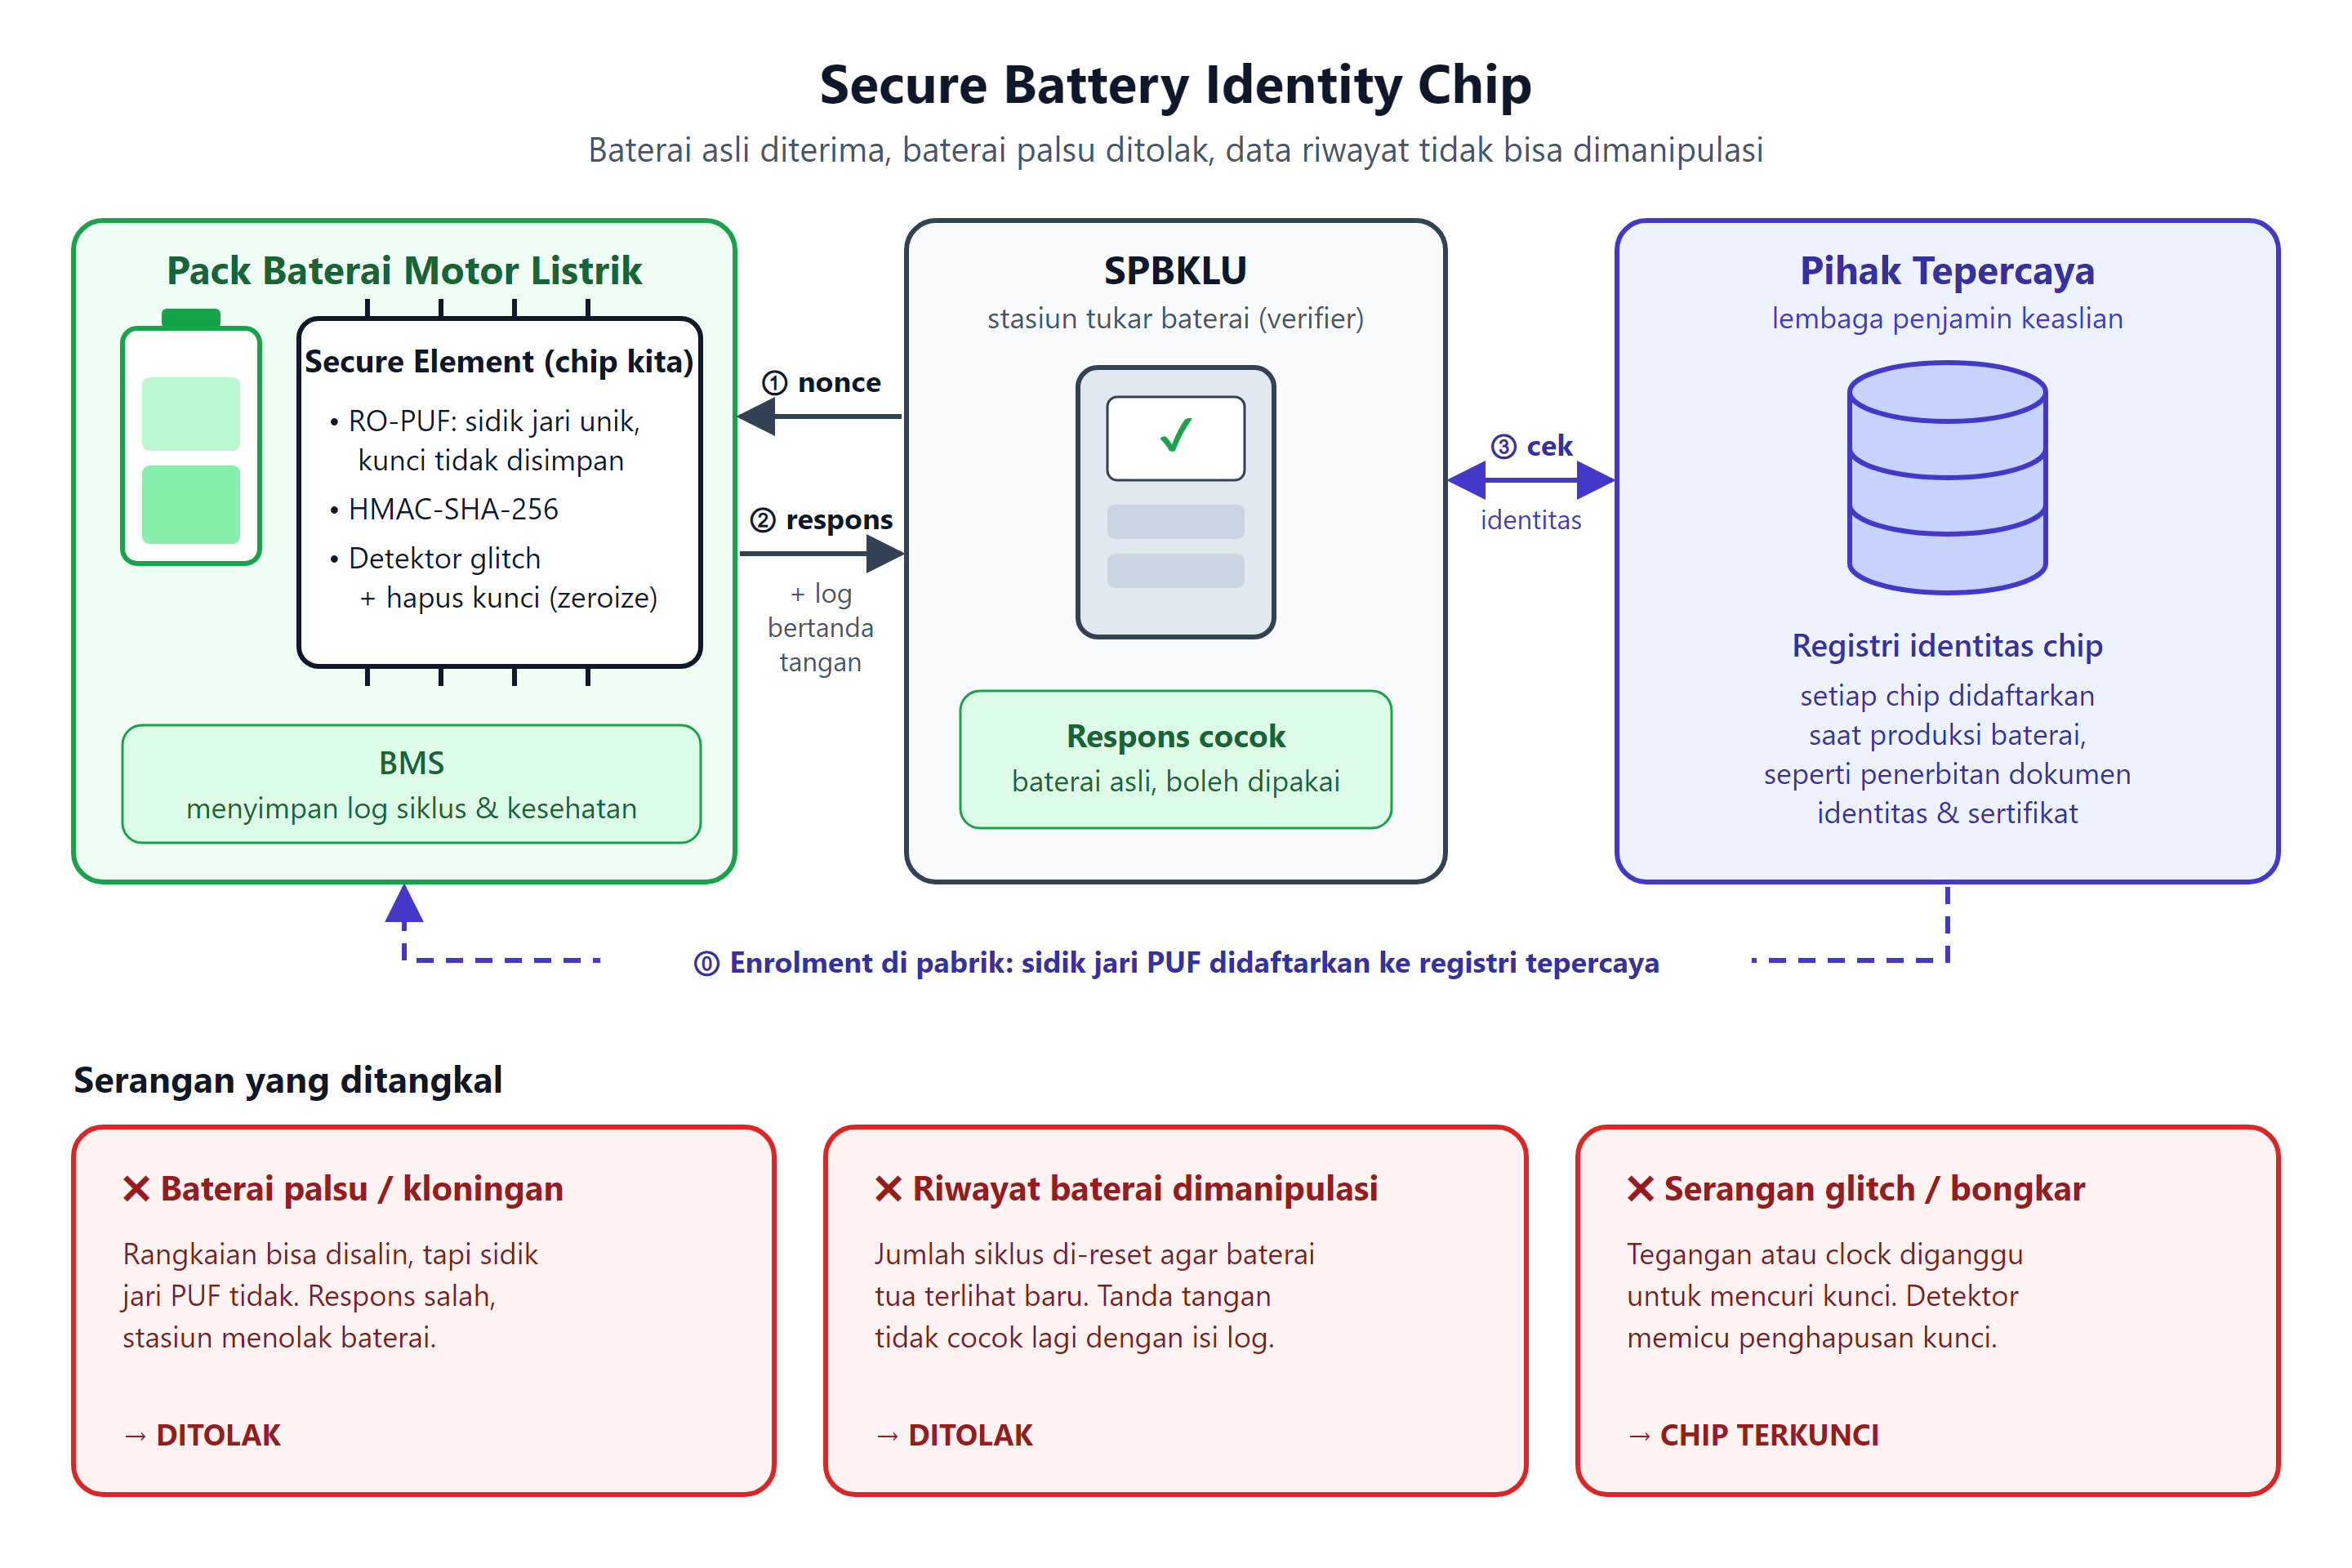
\includegraphics[width=0.95\linewidth]{figures/ilustrasi-ide.png}
  \caption{Alur autentikasi baterai: enrolment di pabrik, \emph{challenge--response} di stasiun tukar baterai, dan serangan yang ditangkal.}
\end{figure}

\field{Implementasi pada DE10-Nano:}
\emph{FPGA fabric} Cyclone~V pada DE10-Nano~\cite{de10} menjalankan seluruh \emph{secure element}: RO-PUF, \emph{fuzzy extractor}, inti HMAC-SHA-256, FSM autentikasi, dan monitor \emph{tamper}. HPS (ARM Cortex-A9, Linux) berperan sebagai \emph{lingkungan uji}: ia mengemulasikan BMS dan stasiun SPBKLU, mengirim perintah melalui \emph{Lightweight HPS-to-FPGA bridge} (AXI), dan memverifikasi respons dengan model referensi Python. Batas antara HPS dan fabric mewakili antarmuka fisik chip (I\textsuperscript{2}C/SMBus pada versi ASIC). Kunci tidak memiliki jalur apa pun ke bus, sehingga HPS yang dibobol pun tidak dapat membacanya. Karena antarmukanya sederhana dan tidak memerlukan memori non-volatil, IP ini juga dapat diintegrasikan sebagai blok tambahan pada baseline chip penyelenggara~\cite{peruri}.

\field{Arsitektur Chip}

\begin{figure}[H]
\centering
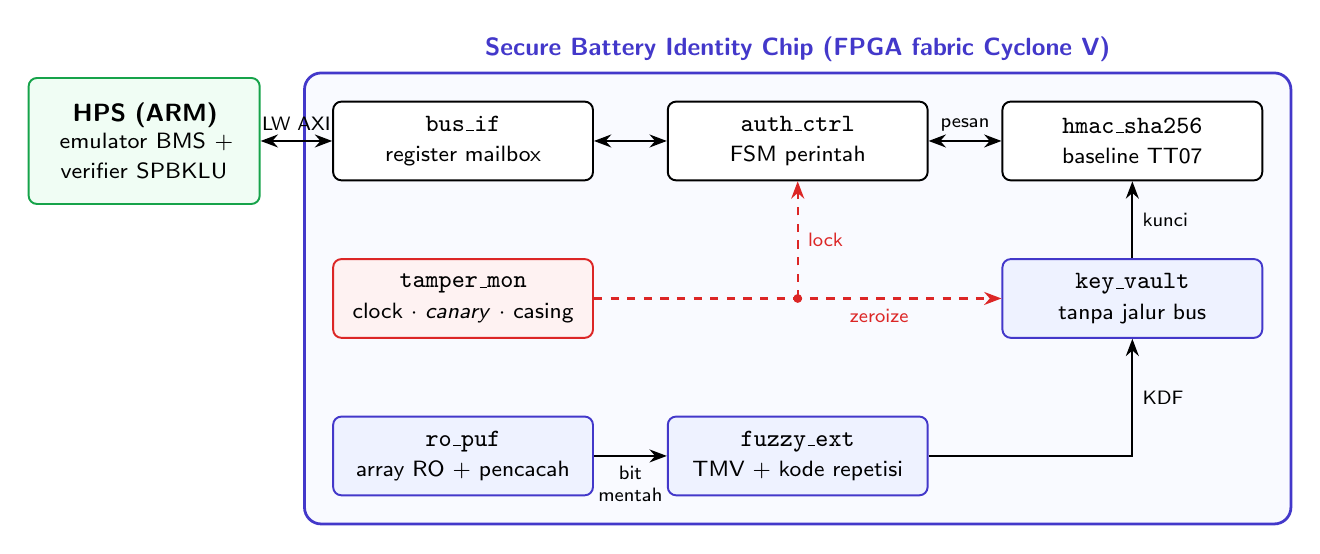
\begin{tikzpicture}[
  font=\sffamily\small,
  blk/.style={draw, rounded corners=3pt, align=center, minimum height=1.0cm, minimum width=3.3cm, fill=white, line width=0.7pt},
  key/.style={blk, fill=secfill, draw=secline},
  mon/.style={blk, fill=badfill, draw=badline},
  host/.style={blk, fill=okfill, draw=okline, minimum width=2.9cm, text width=2.7cm},
  arr/.style={-{Stealth[length=2.2mm]}, line width=0.7pt},
  biarr/.style={{Stealth[length=2.2mm]}-{Stealth[length=2.2mm]}, line width=0.7pt},
  zer/.style={-{Stealth[length=2.2mm]}, line width=0.8pt, draw=badline, dashed},
  lbl/.style={font=\sffamily\scriptsize, align=center}
]
  % Baris 1: jalur perintah
  \node[blk] (bus)  at (0,0)    {\texttt{bus\_if}\\\footnotesize register mailbox};
  \node[blk] (ctrl) at (4.25,0)  {\texttt{auth\_ctrl}\\\footnotesize FSM perintah};
  \node[blk] (hmac) at (8.5,0)  {\texttt{hmac\_sha256}\\\footnotesize baseline TT07};
  % Baris 2: monitor keamanan dan penyimpan kunci
  \node[mon] (tamp)  at (0,-2)   {\texttt{tamper\_mon}\\\footnotesize clock $\cdot$ \emph{canary} $\cdot$ casing};
  \node[key] (vault) at (8.5,-2) {\texttt{key\_vault}\\\footnotesize tanpa jalur bus};
  % Baris 3: pembangkitan kunci
  \node[key] (puf) at (0,-4)   {\texttt{ro\_puf}\\\footnotesize array RO + pencacah};
  \node[key] (fe)  at (4.25,-4) {\texttt{fuzzy\_ext}\\\footnotesize TMV + kode repetisi};
  % Host
  \node[host, minimum height=1.6cm] (hps) at (-4.05,0) {\textbf{HPS (ARM)}\\\footnotesize emulator BMS +\\\footnotesize verifier SPBKLU};

  \begin{scope}[on background layer]
    \node[draw=secline, line width=1pt, rounded corners=6pt, fill=secfill!35, inner sep=10pt,
          fit=(bus)(ctrl)(hmac)(vault)(fe)(puf)(tamp),
          label={[font=\sffamily\small\bfseries, text=secline]above:Secure Battery Identity Chip (FPGA fabric Cyclone V)}] (chip) {};
  \end{scope}

  % Jalur perintah
  \draw[biarr] (hps) -- node[lbl, above]{LW AXI} (bus);
  \draw[biarr] (bus) -- (ctrl);
  \draw[biarr] (ctrl) -- node[lbl, above]{pesan} (hmac);
  % Jalur kunci
  \draw[arr] (puf) -- node[lbl, below]{bit\\mentah} (fe);
  \draw[arr] (fe.east) -- (8.5,-4) -- node[lbl, right]{KDF} (vault.south);
  \draw[arr] (vault) -- node[lbl, right]{kunci} (hmac);
  % Respons serangan
  \draw[zer] (tamp.east) -- node[lbl, below, text=badline, pos=0.7]{zeroize} (vault.west);
  \draw[zer] (4.25,-2) -- node[lbl, right, text=badline]{lock} (ctrl.south);
  \fill[badline] (4.25,-2) circle (1.6pt);
\end{tikzpicture}
\caption{Arsitektur \emph{secure element}. Blok biru menangani kunci dan tidak terhubung ke bus; blok merah adalah monitor keamanan yang menghapus kunci (\emph{zeroize}) dan mengunci FSM (\emph{lock}) saat serangan terdeteksi. \emph{Helper data} PUF bersifat publik dan dibaca melalui \texttt{bus\_if}.}
\end{figure}

\section{Technical Design}

\field{Rincian Modul RTL}

\begin{center}
\small
\begin{tabularx}{\linewidth}{|>{\raggedright\arraybackslash}p{3.0cm}|X|}
\hline
\hdr{Modul} & \hdr{Fungsi} \\ \hline
\texttt{bus\_if} & Register \emph{mailbox} (CMD, STATUS, DATA\_IN[256], DATA\_OUT[256], CHIP\_ID). Antarmuka AXI-Lite ke HPS pada FPGA; I\textsuperscript{2}C/SMBus pada versi ASIC. \\ \hline
\texttt{auth\_ctrl} & FSM perintah: \texttt{GET\_ID}, \texttt{AUTH(nonce)} $\rightarrow$ HMAC$(K, \text{nonce}\,\|\,\text{ID})$, \texttt{SIGN\_LOG(nonce, H(log))} $\rightarrow$ HMAC$(K, \text{nonce}\,\|\,H(\text{log}))$. Menolak perintah saat \emph{lock}. \\ \hline
\texttt{hmac\_sha256} & Inti SHA-256 iteratif~\cite{fips180} (baseline TT07, 1 ronde/siklus) dengan \emph{wrapper} HMAC (ipad/opad) sesuai FIPS 198-1~\cite{fips198}. \\ \hline
\texttt{ro\_puf} & Array \emph{ring oscillator} identik dengan pasangan pembanding dan dua pencacah bersama; menghasilkan $\geq$128 bit respons mentah. Penempatan RO dikunci dengan constraint LogicLock agar simetris. \\ \hline
\texttt{fuzzy\_ext} & \emph{Temporal majority voting} (beberapa pembacaan) + kode repetisi dengan \emph{helper data} publik~\cite{dodis} untuk menghasilkan bit stabil; kunci $K = \text{SHA-256}(\text{bit stabil}\,\|\,\text{label})$. \\ \hline
\texttt{key\_vault} & Register kunci tanpa jalur baca ke bus; diisi saat \emph{boot}, dihapus pada \emph{zeroize}. \\ \hline
\texttt{tamper\_mon} & (1) Monitor frekuensi clock terhadap osilator internal; (2) sensor \emph{canary} berbasis \emph{delay line} yang mendeteksi pelanggaran timing akibat \emph{glitch} tegangan/clock; (3) pin sakelar casing. Pemicu $\rightarrow$ \emph{zeroize} + \emph{lock}. \\ \hline
\end{tabularx}
\end{center}

\field{Protokol Enrolment \& Verifikasi}
\begin{enumerate}
  \item \textbf{Enrolment (pabrik baterai, sekali):} chip menghasilkan \emph{helper data} dan identitas publik. Registri pihak tepercaya mencatat pasangan (ID chip, kunci turunan) melalui kanal produksi yang aman. \emph{Helper data} bersifat publik dan disimpan di BMS.
  \item \textbf{Verifikasi (stasiun, setiap penukaran):} stasiun membuat \emph{nonce} 256-bit dan mengirimkannya ke baterai. Chip membalas dengan respons HMAC dan tanda tangan log. Stasiun meneruskan (ID, \emph{nonce}, respons) ke layanan verifikasi pihak tepercaya, yang menjawab \emph{valid/tidak valid}. Stasiun tidak pernah memegang kunci chip mana pun, sehingga kebocoran satu stasiun tidak membuka seluruh jaringan.
  \item \textbf{Pengembangan lanjutan:} tanda tangan asimetris (ECC, baseline yang juga disediakan panitia) untuk verifikasi luring dengan sertifikat yang diterbitkan otoritas sertifikat tepercaya.
\end{enumerate}

\field{Estimasi Penggunaan Resource FPGA}

Angka berikut adalah \textbf{estimasi awal} berdasarkan ukuran tipikal inti SHA-256 iteratif dan array RO-PUF. Angka final akan diganti dengan hasil sintesis Quartus/Yosys.

\begin{center}
\small
\begin{tabularx}{\linewidth}{|X|X|X|}
\hline
\hdr{Komponen Resource} & \hdr{Estimasi Penggunaan} & \hdr{Kapasitas DE10-Nano} \\ \hline
Logic Elements / LUT & $\approx$3.000--4.500 ALM ($<11\%$) & 110,000 LEs / 41,910 ALMs \\ \hline
Registers / Flip-Flops (FF) & $\approx$2.500--4.000 & 415,000 \\ \hline
Block RAM (M10K) & 0--2 blok (buffer pesan) & 5,570 Kbits \\ \hline
DSP Blocks & 0 & 112 DSP \\ \hline
PLL & 1 (clock sistem) & 6 \\ \hline
\end{tabularx}
\end{center}

Perkiraan latensi: satu blok SHA-256 $\approx$ 65--70 siklus; satu autentikasi HMAC (4 kompresi) $\approx$ 280 siklus, atau $\approx 5{,}6\,\mu$s pada 50~MHz. Regenerasi kunci PUF dilakukan sekali saat \emph{boot} (target $<0{,}5$ s).

\field{Perangkat Lunak \& Tools Perancangan:}
Intel Quartus Prime Lite (sintesis, timing, LogicLock, SignalTap), Platform Designer (integrasi HPS--FPGA), Verilator + cocotb (verifikasi otomatis), Icarus Verilog, Yosys (estimasi area lintas target), Python (model referensi HMAC, verifier, analisis statistik PUF), opsional OpenROAD + SkyWater 130 PDK untuk eksplorasi ASIC.

\subsection{Rencana Pengujian}

\field{Simulasi RTL:}
\begin{itemize}
  \item SHA-256 dan HMAC diuji dengan vektor uji resmi FIPS 180-4 dan RFC 4231~\cite{rfc4231}, dibandingkan bit-per-bit dengan model Python (cocotb).
  \item FSM autentikasi: seluruh perintah, \emph{nonce} berulang, perintah tidak valid, dan perilaku saat \emph{lock}.
  \item \emph{Fuzzy extractor}: injeksi derau bit acak pada respons PUF untuk mengukur batas koreksi.
  \item \emph{Fault injection} di simulasi: membalik bit pada register kunci dan FSM, memastikan chip berakhir dalam keadaan aman.
  \item Pengukuran latensi dan \emph{throughput} dalam siklus.
\end{itemize}

\field{Uji Hardware Board FPGA DE10-Nano:}
\begin{itemize}
  \item Sintesis dan \emph{timing closure}; verifikasi sinyal internal dengan SignalTap (dinonaktifkan pada \emph{build} final agar tidak menjadi jalur kebocoran kunci).
  \item Karakterisasi PUF: pembacaan berulang pada beberapa kondisi (dingin, suhu ruang, dipanaskan) dan beberapa lokasi penempatan RO (serta beberapa board bila tersedia).
  \item Demo serangan: (1) bitstream identik di board lain atau lokasi RO lain $\rightarrow$ ditolak; (2) \emph{replay} respons lama $\rightarrow$ ditolak; (3) log yang diubah $\rightarrow$ ditolak; (4) \emph{glitch} clock melalui rekonfigurasi PLL dan pin \emph{tamper} $\rightarrow$ \emph{zeroize}.
  \item Uji keacakan bit PUF dengan subset NIST SP 800-22~\cite{sp80022}.
\end{itemize}

\field{Metrik Keberhasilan Target:}

\begin{center}
\small
\begin{tabularx}{\linewidth}{|>{\raggedright\arraybackslash}p{4.6cm}|X|}
\hline
\hdr{Metrik} & \hdr{Target / Metode} \\ \hline
Kebenaran kriptografi & 100\% cocok dengan vektor uji FIPS 180-4 / RFC 4231 \\ \hline
Reliabilitas PUF & \emph{Intra-distance} mentah $<10\%$; kunci final 100\% stabil di seluruh kondisi uji \\ \hline
Keunikan PUF & \emph{Inter-distance} mendekati 50\% antarlokasi/antar-board \\ \hline
Latensi autentikasi & $<10\,\mu$s (hardware), terukur dalam siklus \\ \hline
Ketahanan serangan & 4/4 skenario serangan terdeteksi atau ditolak; 0 \emph{false accept} \\ \hline
Efisiensi area & $<15\%$ ALM, 0 DSP, tanpa NVM \\ \hline
Fmax & $\geq$ 50 MHz setelah \emph{timing closure} \\ \hline
\end{tabularx}
\end{center}


\section{Security Design}

\field{Model Ancaman}
Setiap blok chip ada karena satu ancaman nyata:

\begin{center}
\small
\begin{tabularx}{\linewidth}{|>{\raggedright\arraybackslash}p{3.4cm}|X|>{\raggedright\arraybackslash}p{4.1cm}|}
\hline
\hdr{Penyerang \& tujuan} & \hdr{Serangan} & \hdr{Blok penangkal} \\ \hline
Pemalsu baterai & Menyalin rangkaian/firmware chip asli ke baterai palsu & RO-PUF + \emph{fuzzy extractor} (kunci tidak tersimpan) \\ \hline
Penyadap jalur komunikasi & Merekam respons lama lalu mengirim ulang (\emph{replay}) & \emph{Nonce} acak dari stasiun + HMAC-SHA-256 \\ \hline
Operator/bengkel nakal & Me-\emph{reset} jumlah siklus agar baterai tua terlihat baru & Penandatanganan log BMS oleh chip \\ \hline
Penyerang fisik (memegang pack) & \emph{Glitch} clock/tegangan untuk membocorkan atau melewati verifikasi & Monitor clock, sensor \emph{canary} timing, \emph{zeroize} + \emph{lock} \\ \hline
Penyerang fisik & Membongkar casing untuk \emph{probing} & Pin \emph{tamper} (sakelar casing) $\rightarrow$ \emph{zeroize} \\ \hline
Perangkat lunak terkompromi di host & Membaca kunci lewat bus & Tidak ada jalur bus ke register kunci; kunci dihapus setelah dipakai \\ \hline
\end{tabularx}
\end{center}

\textbf{Batasan yang kami akui:} sensor \emph{glitch} tegangan pada FPGA diuji melalui \emph{canary} timing dan rekonfigurasi clock, bukan injeksi tegangan presisi; proteksi \emph{side-channel} (analisis daya~\cite{dpa}) dicatat sebagai ancaman dan pekerjaan lanjutan. Jika PUF belum stabil saat bootcamp, demo dijalankan dengan mode kunci tetap (diungkapkan secara terbuka) sementara karakterisasi PUF dilanjutkan.

% =====================================================================
\clearpage
\section*{Daftar Pustaka}
\vspace{-14pt}
\begin{thebibliography}{99}\small
\bibitem{tt07} Tiny Tapeout, \emph{Tiny Tapeout 7 Datasheet}, 2025. github.com/TinyTapeout/tinytapeout-07
\bibitem{perpres55} Peraturan Presiden RI No.~55 Tahun 2019 tentang Percepatan Program Kendaraan Bermotor Listrik Berbasis Baterai untuk Transportasi Jalan.
\bibitem{perpres79} Peraturan Presiden RI No.~79 Tahun 2023 tentang Perubahan atas Perpres No.~55 Tahun 2019.
\bibitem{ruptl} PT PLN (Persero), \emph{Rencana Usaha Penyediaan Tenaga Listrik (RUPTL) 2025--2034}, hlm.~II-53--II-54.
\bibitem{rukn} Kementerian ESDM, \emph{Rencana Umum Ketenagalistrikan Nasional (RUKN)}, Kepmen ESDM No.~85.K/TL.01/MEM.L/2025, hlm.~51.
\bibitem{barel} H. Bar-El \emph{et al.}, ``The Sorcerer's Apprentice Guide to Fault Attacks,'' \emph{Proceedings of the IEEE}, vol.~94, no.~2, 2006.
\bibitem{suh} G. E. Suh and S. Devadas, ``Physical Unclonable Functions for Device Authentication and Secret Key Generation,'' \emph{Proc. Design Automation Conference (DAC)}, 2007.
\bibitem{maes} R. Maes, \emph{Physically Unclonable Functions: Constructions, Properties and Applications}, Springer, 2013.
\bibitem{de10} Terasic, \emph{DE10-Nano User Manual}.
\bibitem{peruri} PERURI, \emph{Peruri Chip Design Datasheet}, chip.peruri.co.id/datasheet.pdf
\bibitem{fips180} NIST, \emph{FIPS 180-4: Secure Hash Standard (SHS)}, 2015.
\bibitem{fips198} NIST, \emph{FIPS 198-1: The Keyed-Hash Message Authentication Code (HMAC)}, 2008.
\bibitem{dodis} Y. Dodis, L. Reyzin, and A. Smith, ``Fuzzy Extractors: How to Generate Strong Keys from Biometrics and Other Noisy Data,'' \emph{EUROCRYPT}, 2004.
\bibitem{rfc4231} M. Nystrom, \emph{RFC 4231: Identifiers and Test Vectors for HMAC-SHA-224, -256, -384, and -512}, IETF, 2005.
\bibitem{sp80022} NIST, \emph{SP 800-22 Rev.~1a: A Statistical Test Suite for Random and Pseudorandom Number Generators}, 2010.
\bibitem{dpa} P. Kocher, J. Jaffe, and B. Jun, ``Differential Power Analysis,'' \emph{CRYPTO}, 1999.
\end{thebibliography}

% =====================================================================
\clearpage
\section*{Lampiran Teknis}

\begin{itemize}
  \item Repositori proyek (RTL, testbench, model Python, dokumentasi): \todo{tautan GitHub, atur akses bila perlu dibagikan ke juri}.
  \item Diagram alur sistem (Gambar 1) dan arsitektur chip (Gambar 2).
  \item Register map dan spesifikasi perintah \texttt{auth\_ctrl} (dilengkapi pada laporan teknis).
\end{itemize}

\section*{Tim \& Pembagian Peran}

\begin{center}
\small
\begin{tabularx}{\linewidth}{|>{\raggedright\arraybackslash}p{3.6cm}|>{\raggedright\arraybackslash}p{3.6cm}|X|}
\hline
\hdr{Nama Anggota} & \hdr{Keahlian Utama} & \hdr{Tanggung Jawab \& Peran} \\ \hline
Guntur Sulistyo (Ketua) & Security / Safety Analyst & Model ancaman, desain \texttt{tamper\_mon} dan respons \emph{fail-secure}, skenario serangan dan \emph{fault injection}, karakterisasi PUF, koordinasi tim. \\ \hline
Dimas Eryan Ahnaf Fahrezi & System / Business Analyst & Kebutuhan sistem ekosistem SPBKLU, protokol enrolment dan registri identitas, model referensi Python dan verifier, dokumentasi dan presentasi. \\ \hline
Muhammad Muqtada Alhaddad & RTL Designer / Verilog & Integrasi SHA-256 TT07 dan HMAC, \texttt{ro\_puf}, \texttt{fuzzy\_ext}, \texttt{auth\_ctrl}, integrasi HPS--FPGA, sintesis dan \emph{timing}. \\ \hline
\end{tabularx}
\end{center}

\section*{Luaran \& Demo (Opsional)}

\field{Demo Live:}
Dua ``baterai'' (board atau lokasi PUF berbeda) diuji di stasiun emulasi: baterai asli diterima, kloningan ditolak, log yang dimanipulasi ditolak, dan \emph{glitch} clock atau pembukaan ``casing'' memicu \emph{zeroize} dengan indikator LED.

\field{Video Demo:}
Video 3--5 menit: masalah baterai palsu, arsitektur chip, alur enrolment--verifikasi, dan empat skenario serangan.

\field{Repository Source Code:}
RTL Verilog, testbench cocotb, model referensi Python, proyek Quartus/Platform Designer, skrip karakterisasi PUF, dan bitstream (.sof/.rbf).

\field{Laporan Teknis Singkat:}
Spesifikasi arsitektur dan register map, hasil sintesis/timing/resource, statistik PUF (keunikan, reliabilitas, keacakan), latensi autentikasi, dan hasil uji serangan.

\section*{Rencana Bootcamp (3 Hari) (Opsional)}

\field{Jadwal \& Target Eksekusi:}

\begin{center}
\small
\begin{tabularx}{\linewidth}{|>{\centering\arraybackslash}p{1.6cm}|>{\raggedright\arraybackslash}p{4.8cm}|X|}
\hline
\hdr{Hari} & \hdr{Fokus Kegiatan} & \hdr{Target Deliverables} \\ \hline
\textbf{Hari 1} & Integrasi inti \& masukan mentor & HMAC-SHA-256 lolos vektor uji di board; FSM autentikasi terhubung ke HPS; respons PUF mentah terbaca. \\ \hline
\textbf{Hari 2} & Kunci PUF \& keamanan & \emph{Fuzzy extractor} menghasilkan kunci stabil; \texttt{tamper\_mon} + \emph{zeroize} aktif; statistik PUF dan resource/timing terukur. \\ \hline
\textbf{Hari 3} & Validasi \& demo & Empat skenario serangan berjalan; video demo; laporan teknis dan materi presentasi final. \\ \hline
\end{tabularx}
\end{center}

\end{document}
